\section{Introduction}

To compile this document, run the following commands: 

\begin{verbatim}
prompt> latex latex-for-class
prompt> bibtex latex-for-class
prompt> latex latex-for-class
prompt> latex latex-for-class
prompt> dvips -o latex-for-class.ps latex-for-class
prompt> ps2pdf latex-for-class.ps
\end{verbatim}

This will create the latex-for-class.pdf file. You have to run latex a
couple of times to get cross-references resolved. 

\subsection{Math Symbols}

This is {\it italics}, {\bf bold font}. This is how we use math mode:

\begin{align}
A = a_0 + a_1 \alpha + a_2 \alpha^2 = \sum _{i=0}^{2} a_i \cdot \alpha^i
\end{align}

This is also how to use in-line math mode: $\F, \R, \Q, \C, \Fq,
\Fkk$, based on my macros.

Let $ \idealj = \idealg \subseteq \Fq[x_1, \dots, x_n]$ and let $V(J)$
denote the variety $V$ of ideal $J$. Actually, since variety is needed
over $\Fq$ itself, use $\vfqj$.

This is how you write an algorithm and refer to it as
Alg. \ref{alg:gb}, see the caption below the algorithm description in
the intro.tex file.

\begin{algorithm}[hbt]
\SetAlgoNoLine
 \KwIn{$F = \{f_1, \dots, f_s\}$}
 \KwOut{$G = \{g_1,\dots ,g_t\}$\\} %, a Gr\"{o}bner basis
  $G:= F$\;
  \Repeat{$G = G'$}
  {
  	$G' := G$\;
  	\For{ each pair $\{f, g\}, f \neq g$ in $G'$} 
	{
		$Spoly(f, g) \stackrel{G'}{\textstyle\longrightarrow}_+r$ \;
		\If{$r \neq 0$}
		{
			$G:= G \cup \{r\}$ \;
		}
	}
   }
\caption {Buchberger's Algorithm}
\label{alg:gb}
\end{algorithm}

This is how you write the polynomial reduction of $f \pmod{ G}: f
\xrightarrow{g_1, \dots, g_t} _+ r$ where $G = \{g_1, \dots,
g_t\}$. Also, there are many ways to write a matrix, two of them are: 

\[
M = \begin{pmatrix*}[l]
 & x^2y & y^3 & y^2 & y\\
f_4 & \frac{1}{3} & \frac{1}{2} & 0 & 0 \\
yf_1 & 2 &0 & 1 & 0 \\
yf_3 & 0 & 4 & 0 & -1
\end{pmatrix*}
\]

\[
M = \bordermatrix{
~ & x^2y & y^3 & y^2 & 1\cr
f_4 & \frac{1}{3} & \frac{1}{2} & 0 & 0 \cr
yf_1 & 2 &0 & 1 & 0 \cr
f_3 & 0 & 4 & 0 & -1 \cr
}
\]

Now, reducing $M$ to a row echelon form using Gaussian elimination gives:
\[
M = \bordermatrix{
~ & x^2y & y^3 & y^2 & 1\cr
f_4 & \frac{1}{3} & \frac{1}{2} & 0 & 0 \cr 
h = f_4 - \frac{1}{6}yf_1 & 0 &\frac{1}{3}  & -\frac{1}{6} & 0 \cr 
r = h - \frac{1}{8}f_3 & 0 & 0 & -\frac{1}{6} & \frac{1}{8} \cr 
}
\]


This is how you provide citation for a journal paper \cite{ted_tcomp},
conference paper \cite{shekhar:fmcad06}, book \cite{ideals:book} or a
PhD thesis \cite{buchberger_thesis}.  

\begin{Theorem}
This theorem states that Prof. Kalla is indeed the best.
\end{Theorem}

\begin{Proof}
The proof is trivial.
\end{Proof}

\begin{Corollary}
No one is better than Prof. Kalla.
\end{Corollary}

Finally, this is how you include a figure as shown in Fig. \ref{fig:ckt}. 

\begin{figure}[hbt]
\centering
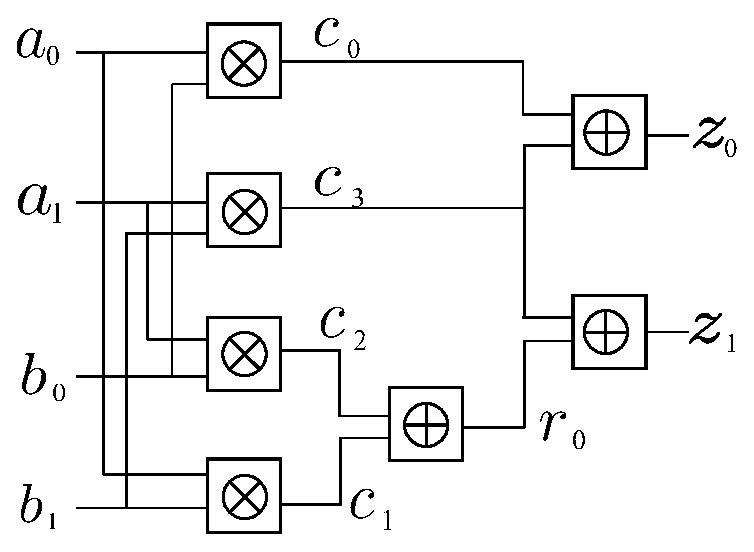
\includegraphics[scale=0.5]{2bitmultiplier.eps}
\caption{This is a figure}
\label{fig:ckt}
\end{figure}